\documentclass[../CAP6619_term_project_cgarbin.tex]{subfiles}

\begin{document}

\subsection{Datasets}

Tests were performed on two image classification datasets, MNIST \cite{LeCun1999} and CIFAR-10 \cite{Krizhevsky2009}.

\medskip
\textbf{MNIST}

MNIST \cite{LeCun1999} is a set of 60,000 training and 10,000 test images of handwritten digits from 0 to 9. All images are 28x28 pixels in grayscale, with the digits centered in the image.

Although it is sometimes mentioned as the "postal (ZIP) code" set, it was not created from actually posted letters. It was created by combining a subset of two NIST digit sets, one containing digits from employees of the Census Bureau, and one containing digits from high-school students. These sets were chosen to provide a mix of samples that are considered easy to classify (the ones from the Census Bureau employees) and samples that are relatively harder to classify (the ones from the high-school students).

To make the validation process more meaningful the training and test sets were split by the original writers in a way that they do not overlap (digits from a given writer are either in the training set or the test set, but not in both) and the two types of writers are equally represented (half of the samples in the training and test set comes from the Census Bureau employees, the other half from the high-school students). This careful split results in a robust evaluation of a trained model (it will be presented with samples from writers it has not been trained on).

Figure~\ref{fig:MnistSample} shows a sample of the MNIST dataset.

\begin{figure}[!htbp]
\centerline{\includegraphics[width=0.9\columnwidth]{figures/figures_other/MnistExamples.png}}
\caption{MNIST sample digits \cite{Steppana}}
\label{fig:MnistSample}
\end{figure}

\medskip
\textbf{CIFAR-10}

CIFAR-10 \cite{Krizhevsky2009} is a set of 50,000 training and 10,000 test images. All images are 32x32 pixels in color (RGB channels).

It contains 10 classes of images. The training set has 5,000 images of each class. The test set has 1,000 images of each class.

The set was created from images collected from the internet and manually labeled by humans. The creation process ensured that no duplicates or synthetically-created images are present in the set.

Figure~\ref{fig:CifarSample} shows a sample of the CIFAR-10 dataset.

\begin{figure}[!htbp]
\centerline{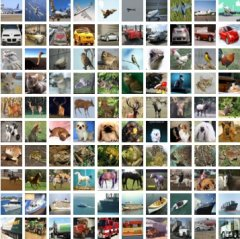
\includegraphics[width=0.9\columnwidth]{figures/figures_other/cifar10.jpeg}}
\caption{CIFAR-10 sample pictures \cite{Karpathy}}
\label{fig:CifarSample}
\end{figure}

\subsection{Dropout}

Dropout \cite{Srivastava2014} is a technique to reduce overfitting. Its central idea is to take a model that is overfitting and train sub-models derived from it by randomly removing units for each training batch. See figure~\ref{fig:DropoutHowItWorks}.

\begin{figure}
\centerline{\includegraphics[width=0.9\columnwidth]{figures/figures_other/DropoutHowItWorks.png}}
\caption{How dropout works: randomly removing units from a fully connected network (left) to create a sub-model (right). Original picture from \cite{Srivastava2014}.}
\label{fig:DropoutHowItWorks}
\end{figure}

By repeatedly eliminating random units, Dropout forces the units to be more robust, learning feature on their own, without depending on other units. In this context it can be thought of as simplified model-ensembling.

The number of units to retain is controlled by a new hyperparameter, the \textit{dropout rate}.\footnote{Note that the Keras API use this parameter to control the number of units to \textit{remove} (the opposite meaning of what is used in the Dropout paper). This paper follows the Keras API, i.e. units to remove.} The recommended values for the dropout rate are 0.1 for the input layer and between 0.5 and 0.8 for internal layers.

Using Dropout requires some adjustments to the hyperparameters. The more significant changes are:

\begin{itemize}
\item Increase the network size: Dropout removes units during training reducing the capacity of the network. To compensate for that the number of units has to be adjusted by the dropout rate, i.e. the number of units has to be multiplied by 1/(dropout rate). For example, if the dropout rate is 0.5, it will double the number of units.
\item Increase learning rate and momentum: dropout introduces noise in the gradients, causing them to cancel each other sometimes. Increasing the learning rate by 10-100x and adding momentum between 0.95 and 0.99 compensates that effect.
\item Add max-norm regularization: increasing the learning rate and adding momentum may result in large weight values. Adding max-norm regularization counteracts that effect.
\end{itemize}

When applying these rules, note that the paper seems to have tested these guidelines with a regular, non-adaptive SGD optimizer. They may not apply exactly as described for adaptive optimizers.

\subsection{Batch Normalization}

During training of a neural network the distribution of the input values of each layer is affected by all layers that come before it. This variability reduces training speed (lower learning rates). Batch Normalization \cite{Ioffe2015} was created to resolve this variability and speed up learning.

Normalizing the values of each sample before presenting it to the network's input layer was already a well-known technique. Batch Normalization goes one step further and normalizes the input in every layer of the network, not only the input layer. The normalization is computed for each batch. This normalization allows the use of higher learning rates during training (although the paper does not recommend a specific value or a range).

The way Batch Normalization operates, by adjusting the value of the units for each batch, and the fact that batches are created randomly during training, results in more noise during the training process. The noise acts as a regularizer. This regularization effect is similar to the one introduced by Dropout. As a result, Dropout can be removed completely from the network or should have its rate reduced significantly if used in conjunction with Batch Normalization.

Using Batch Normalization requires some adjustments to the hyperparameters. The more significant changes are:

\begin{itemize}
\item Increase the learning rate: the normalization stabilizes the training process, allowing higher learning rates.
\item Remove Dropout or use lower dropout rates: Batch Normalization also has a regularization effect. This effect reduces the need for Dropout to the point it is no longer needed. If it is used, it should be used with lower dropout rates. 
\end{itemize}


\subsection{Network Configurations}

In this report we tested multilayer perceptron networks (MLPs) and convolutional neural networks (CNNs) with different hyperparameter configurations.

\medskip
\textbf{Multilayer Perceptron Network Tests}

Multilayer perceptron networks are networks composed of several fully connected layers.  An example is shown in figure~\ref{fig:MlpStandardModel}.

The MNIST dataset was used to test the MLP networks and hyperparameters combinations. MNIST was chosen for this test because the original Dropout paper \cite{Srivastava2014} also used MNIST in their MLP tests and formulated their guidelines for hyperparameters based on that. The Dropout paper recommends ranges of values for hyperparameters, including number of layers (2 to 4), number of units in the hidden layer (1024 to 4096 and a special case of 8192), learning rate (10x to 100x what would normally be used without Dropout), max-norm (3 to 4), among others.

We tested these combinations to document the effect they have on the network. The goal is to test combinations of the recommendations from that paper, verifying how they affect the training performance and the accuracy of the training model of an MLP network.

\medskip
\textbf{Convolutional Neural Network Tests}

Convolutional neural networks are networks composed of several convolution and max-pooling layers. An example is shown in figure~\ref{fig:CnnStandardModel}.

CNN was used to test the CIFAR-10 dataset in the Dropout paper \cite{Srivastava2014}. The Batch Normalization paper \cite{Ioffe2015} used the ImageNet dataset for a similar test. For simplicity, given the hardware and time available for the tests performed here, CIFAR-10 (instead of ImageNet) was used for the Batch Normalization tests. Since the goal is to compare the relative performance of the strategies and hyperparameters, using CIFAR-10 should suffice in this application.

\subsection{Data Collected}

For each experiment, the following measurements were collected.

\smallskip
\textit{Training CPU time}
\begin{itemize}
\item What it measures: how much time was used across all CPUs and GPUs to run all training epochs.
\item Goal: measure how much system resources a network configuration uses during the training phase. 
\item Why it was measured: to understand how taxing the training phase is for a network configuration. Lower values are desirable to allow efficient use of expensive GPUs and to speed up the experimental phase, where different hyperparameter combinations have to be tried to find an optimal one.
\item How it was measured: with the Python \verb|time| package, measuring the time to it took to execute Keras' \verb|model.fit(...)| function for the network configuration.
\item Note: in systems with more than one CPU or GPU this is not the same as clock (wall) time. Using a simplified example: if a network needs 20 seconds to be trained, in a system with two CPUs the training will complete in about 10 seconds. This item will report 20 seconds in this case. Measuring total CPU and GPU utilization gives a better view of the utilization of systems resources. Measuring only the clock time (10 seconds in this example) would not give an idea of how taxing the training phase really is on the system.
\end{itemize}

\smallskip
\textit{Test CPU time}
\begin{itemize}
\item What it measures: how much time was used across all CPUs and GPUs to evaluate the trained network using the test set.
\item Goal: measure how much system resources the trained network uses when it is evaluating samples. 
\item Why it was measured: to understand how efficient (or not) the trained network is on the end-users' systems. Lower variables are desirable here to be responsive to the end-user and, perhaps more importantly nowadays, to make efficient use of batteries in portable devices (e.g. phones).
\item How it was measured: with the Python \verb|time| package, measuring the time to it took to execute Keras' \verb|model.evaluate(...)| function on the trained network.
\item Note: similarly to the training CPU time, this is not the same as clock (wall) time. See the note for that item for more details.
\end{itemize}

\smallskip
\textit{Number of parameters in the model}
\begin{itemize}
\item What it measures: the number of parameters the model has.
\item Goal: measure how much memory the model uses.
\item Why it was measured: to have a second parameter to decide among models that have the same accuracy. The model with fewer parameters should be used because it will be faster to experiment with (run more training experiments), will use less memory on an end-user's device (and thus contribute to overall performance device by not forcing the operating system to eject other processes from memory) and use less battery (because it executes fewer calculations to predict the output.
\item How it was measured: with Keras' \verb|model.count_params()| function, called on the model object after all layers have been created. Note that this number includes non-trainable parameters, such as auxiliary variables used in Batch Normalization. Therefore size at test time is an approximation (but it is close enough).
\end{itemize}

\smallskip
\textit{Training and validation loss and accuracy for each epoch}
\begin{itemize}
\item What it measures: the training loss shows if the network is improving as training progresses and how fast it is doing so. The validation loss checks if the network is overfitting or underfitting.
\item Goal: measure how fast the network converges and if the network will perform well on unseen data.
\item Why it was measured: to have a measurement for training efficiency among the models tested. Given two models that have the same accuracy, the one that achieves that accuracy faster (fewer epochs) saves system resources at training time (assuming a technique to decide that in real-time, such as early stopping, is being used) and allows faster experimentation cycles.
\item How it was measured: by setting the parameter \verb|validation_data| when executing Keras' \verb|model.fit(...)|. Keras returns a \verb|History| object when validation data is supplied. This object contains the training and validation loss and accuracy for each training epoch. Note that the code uses the test portion of the datasets for this purpose. Since the code is not making decisions based on that (e.g. early stopping \cite{Morgan1989} or annealing the learning rate), this is an acceptable practice. \cite{KerasTeam2016} has a similar discussion for this usage pattern in the Keras examples.
\end{itemize}


\end{document}

% Main body: In the body of your project, you will need to provide technical details of
% your design [ 2000-2500 words: 8 pts]
% b. If your report is about experimental studies, you will need to provide a brief
% description about your learning/classification methods, the benchmark datasets, and
% different measures applied.
% You should also explain how the experiments are carried out in your study, and what type 
% of empirical study goals you intend to achieve.
